
\section{Experiment 2: Zener Diode as Voltage Regulator}

\subsection{Objective}
The objective of this experiment is to study the voltage regulation characteristics of a Zener diode and demonstrate its use in maintaining constant output voltage despite input variations.

\subsection{Theory}
A Zener diode is a special type of diode designed to operate in the reverse breakdown region. In this region, the voltage across the diode remains nearly constant over a wide range of currents, making it useful for voltage regulation.

The Zener voltage \(V_Z\) is the voltage at which breakdown occurs. For currents above the knee current \(I_{ZK}\), the voltage remains approximately constant at \(V_Z\).

Zener diodes are used in voltage regulator circuits to provide a stable reference voltage or to regulate the output voltage of a power supply.

\subsubsection{Applications}
- Voltage regulation in power supplies
- Reference voltage sources
- Overvoltage protection

\subsubsection{Waveforms}
In a Zener regulator, the input voltage varies, but the output across the Zener diode remains constant.

\subsection{Apparatus}
- Zener diode (e.g., 5.1V)
- Variable DC power supply
- Resistor (load resistor)
- Multimeter (for voltage measurement)
- Connecting wires
- Breadboard

\subsection{Schematic Diagrams}
\subsubsection{Zener Voltage Regulator Circuit}
\begin{figure}[H]
    \centering
    \begin{circuitikz}
        \draw (0,0) to [V, v=$V_{in}$] (0,2);
        \draw (0,2) to [R, l=$R_S$] (2,2);
        \draw (2,2) to [diode, l=$D_Z$] (2,0);
        \draw (2,0) to (0,0);
        \draw (2,2) to [R, l=$R_L$] (4,2);
        \draw (4,2) to (4,0);
        \draw (2,0) to [voltmeter] (4,0);
    \end{circuitikz}
    \caption{Zener diode voltage regulator circuit.}
    \label{fig:zener_circuit}
\end{figure}

\subsection{Scaled Graphs}
The regulation characteristic showing output voltage vs input voltage.

\begin{figure}[H]
    \centering
    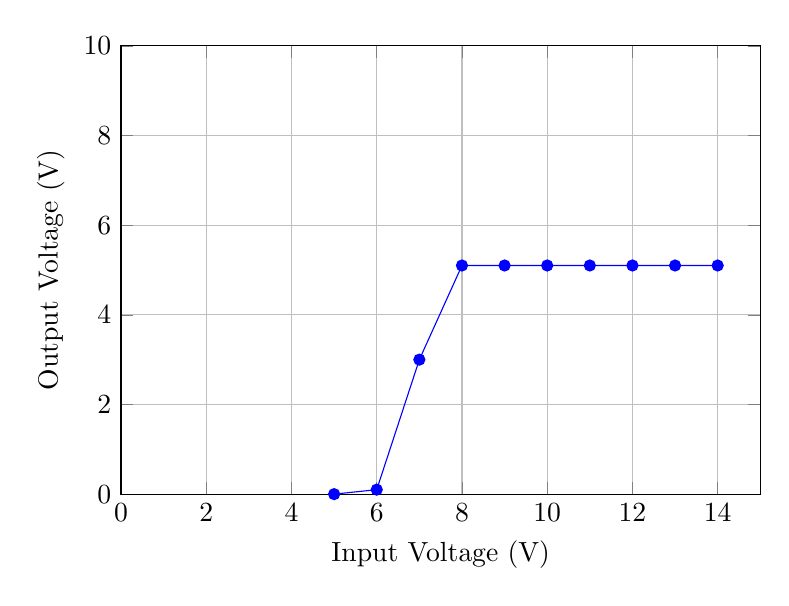
\begin{tikzpicture}
        \begin{axis}[
            width=0.8\textwidth,
            height=0.6\textwidth,
            xlabel={Input Voltage (V)},
            ylabel={Output Voltage (V)},
            grid=both,
            xmin=0, xmax=15,
            ymin=0, ymax=10
        ]
        \addplot[blue, mark=*] coordinates {
            (5, 0)
            (6, 0.1)
            (7, 3)
            (8, 5.1)
            (9, 5.1)
            (10, 5.1)
            (11, 5.1)
            (12, 5.1)
            (13, 5.1)
            (14, 5.1)
        };
        \end{axis}
    \end{tikzpicture}
    \caption{Zener diode regulation characteristic (sample data).}
    \label{fig:zener_plot}
\end{figure}

\subsection{Observations}
The following table shows the input and output voltages for the Zener regulator.

\begin{table}[H]
    \centering
    \caption{Zener Regulator Measurements}
    \begin{tabular}{|c|c|}
        \hline
        Input Voltage (V) & Output Voltage (V) \\
        \hline
        5 & 0 \\
        \hline
        6 & 0.1 \\
        \hline
        7 & 3 \\
        \hline
        8 & 5.1 \\
        \hline
        9 & 5.1 \\
        \hline
        10 & 5.1 \\
        \hline
        11 & 5.1 \\
        \hline
        12 & 5.1 \\
        \hline
        13 & 5.1 \\
        \hline
        14 & 5.1 \\
        \hline
    \end{tabular}
    \label{tab:zener_obs}
\end{table}

\subsection{Discussion}
The results show that once the input voltage exceeds the Zener voltage (5.1V), the output voltage stabilizes at approximately 5.1V, demonstrating effective voltage regulation. Below the breakdown voltage, the diode behaves like a regular diode with low voltage drop. This characteristic makes Zener diodes ideal for maintaining constant voltage in circuits.

\subsection{Conclusion}
The experiment successfully demonstrated the voltage regulation capability of the Zener diode. The objectives were met, showing how Zener diodes can provide stable output voltage for varying inputs, essential for reliable electronic systems.

\section{References}
Sedra, A. S., \& Smith, K. C. (2016). Microelectronic Circuits (7th ed.). Oxford University Press.